\chapter{Interface pelo terminal}
\minitoc

Tendo em vista a facilidade, para alguns utilizadores, em manusear um sistema por um terminal, decidiu-se criar uma interface para a aplicação desenvolvida. Esta interface, 
ainda em fase de desenvolvimento, vai permitir, essencialmente, trabalhar com a base de dados do sistema. Os objectivos passam por consultar listas de determinadas entidades, 
desde \texttt{enunciados} a utilizadores do sistema. De realçar que este modo de comunicação com o sistema apenas é utilizado pelos \textbf{administradores}\\

\section{Perl}

Como linguagem de desenvolvimento para esta interface, decidiu-se usar \texttt{Perl} devido à rapidez de implementação (visto que a criação de uma interface pelo terminal não 
constituía um dos principais objectivos) e a vasta diversificação de módulos existentes para auxílio ao desenvolvimento. Desses módulos, destaca-se o uso do módulo 
\texttt{DBIx::Class}, um módulo de comunicação a base de dados (apresentado durante as aulas de EL::PLN), 
que basicamente representa em classes cada tabela existente na base de dados, transformando também simples \texttt{querys} em métodos sobre as tabelas.\\

Tem-se em vista também a utilização dos seguintes módulos:

\begin{description}
 \item[Digest::SHA2] módulo necessário para ser possível criar um utilizador. A utilização deste módulo servirá para cifrar a \texttt{password} para posteriormente guardar na base de dados.
Escolheu-se este módulo por ser compatível com uma \texttt{gem}, com o mesmo nome, da ferramenta \texttt{Rails}
 \item[Term::ReadLine] módulo que se pretende usar para substituir os menus clássicos, como se pode ver na secção seguinte, por um sistema actual por comandos e histórico.
 \item[XML::DT] módulo que se irá usar para a transformação de enunciados em \texttt{XML} para \texttt{Latex} e para a inserção na base de dados. 
\end{description}

\section{Fase 1}

Na fase actual desta interface, o utilizador desta interface terá pela frente um menu principal (Figura~\ref{img:menuprinc}). \\

\begin{figure}[H]
\begin{center}
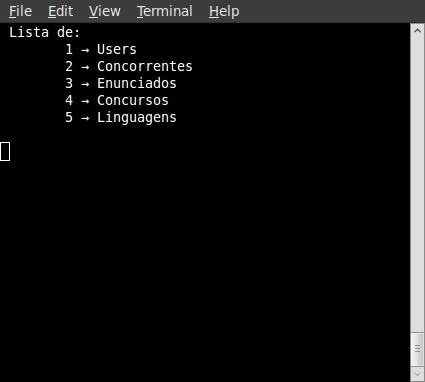
\includegraphics[width=0.45\textwidth]{Images/menuPrinc}
\caption{Menu Principal}\label{img:menuprinc}
\end{center}
\end{figure} 

Cada escolha desse menu representa as principais acções que se podem efectuar com uma base de dados: 

\begin{itemize}
 \item A listagem de elementos
 \item A procura de certos elementos e posterior actualização dos mesmos
 \item A inserção de novos elementos
\end{itemize}

Assim, caso o utilizador escolha a primeira opção, será levado para um novo menu contendo as 5 principais entidades deste sistema: Os \texttt{Users}; os \texttt{Enunciados}; as \texttt{Concorrentes}; os \texttt{Concursos}; e as \texttt{Linguagens} disponíveis para responder em cada concurso. A título de exemplo, caso o utilizador quisesse saber 
as linguagens disponíveis, a informação seria apresentada da seguinte forma(Figura~\ref{img:linguagens}):\\

\begin{figure}[H]
\begin{center}
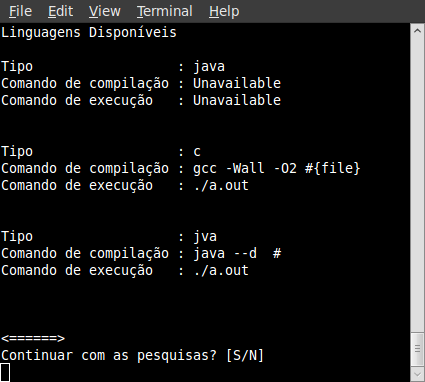
\includegraphics[width=0.45\textwidth]{Images/linguagens}
\caption{Linguagens disponíveis}\label{img:linguagens}
\end{center}
\end{figure} 

O utilizador também poderia procurar por um único elemento. Como se pode ver na Figura~\ref{img:zelladouglas}, dando um nome de utilizador, 
seria retornada a informação sobre esse sujeito. Caso pretendesse, o utilizador poderia posteriormente proceder à alteração do mesmo.\\

\begin{figure}[H]
\begin{center}
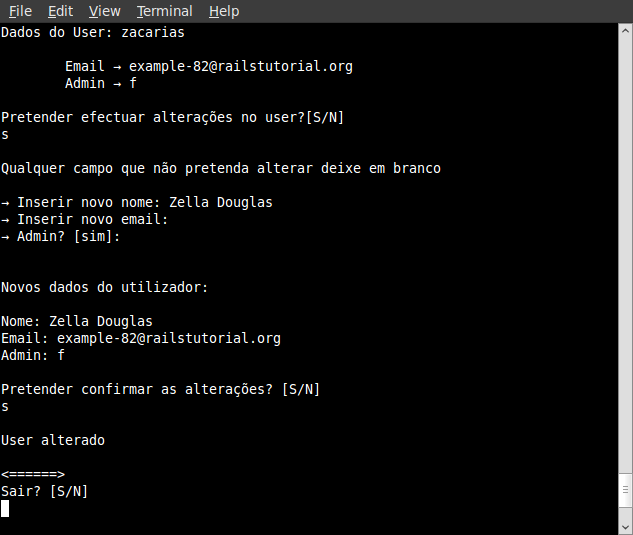
\includegraphics[width=0.65\textwidth]{Images/zacarias}
\caption{Procura e alteração do \texttt{user} Zella Douglas}\label{img:zelladouglas}
\end{center}
\end{figure} 

